\chapter{Introducción}\label{cap.introduccion}
En este primer capítulo se tratará de explicar el contexto de las bases tecnológicas en las que se apoya este proyecto, que son principalmente las tecnologías web y la robótica. Para empezar se hablará sobre el estado actual de la robótica y la gran expansión de la misma en nuestros días. Se continuará señalando el contexto de las tecnologías web y como de importantes son en la sociedad actual, para continuar explicando su arquitectura y las tecnologías más importantes. Para finalizar este capitulo, se introducirá en Jderobot y en los proyectos previos que combinan tecnologías web con componentes robóticos.

\section{Robótica}
El diccionario de la Real Academia Española define robótica como la técnica que aplica la informática al diseño y empleo de aparatos que, en sustitución de personas, realizan operaciones o trabajos, por lo general en instalaciones industriales. El termino robótica proviene del escritor y profesor de bioquímica Isaac Asimov, quien, en su Saga de la Fundación, definió las leyes de la robótica:
\begin{itemize}
	\item Primera ley: Un robot no puede hacer daño a un ser humano ni, por inacción, permitir que un ser humano sufra daño.
	\item Segunda ley: Un robot debe obedecer las órdenes dadas por los seres humanos, excepto cuando estas entren en conflicto con la primera ley.
	\item Tercera ley: Un robot debe proteger su propia integridad, siempre y cuando esto no impida el cumplimiento de la primera y segunda ley.
\end{itemize}
Desde que Asimov acuñara estas tres leyes, la sociedad ha temido lo que los robots puedan hacer al ser humano, desde esclavizarnos hasta quitarnos el trabajo, siendo este miedo el más reciente y el que ha supuesto un mayor freno al desarrollo. Sin embargo, con el paso del tiempo, nos hemos dado cuenta que la robótica tiene una gran utilidad para hacer avanzar la sociedad. Ya no solo pensamos en robótica como en un humanoide que pueda reemplazar al ser humano como nos muestran tantas obras literarias y cinematográficas, sino que vemos robótica a lo largo de nuestro día a días, desde un brazo mecánico en una cadena de montaje, hasta un aspirador robótico. Gracias a la robótica, tareas hasta hoy conllevaban riesgos para la salud humana como la desactivación de artefactos explosivos o trabajos con altas temperaturas, o tareas pesadas y repetitivas se pueden realizar de manera más eficiente y fácil gracias a la robotización de las mismas.

Todo robot debe tener una parte hardware (el componente robótico ya sea real o simulado) y una parte software (la lógica de ese componente robótico).

\subsection{Robótica en la actualidad}
El uso de la robótica en la actualidad está muy extendido, tareas tales como montajes en cadena en una fabrica, trabajos repetitivos de gestión de proyectos o manipulación de objetos peligrosos, ya están robotizados de manera que el ser humano no se ponga en peligro o mal gaste tiempo de manera innecesaria. A continuación se muestra varios ejemplos de uso de la robótica en nuestros días:
\begin{itemize}
\item Cirugía: Los robots se están empezando a usar en procedimientos quirúrgicos, ya que compensan las deficiencias y limitaciones del ser humano en la exactitud y precisión. Además, posibilitan realizar la llamada ``telecirugía'', que se trata de la realización de intervenciones quirúrgicas de manera remota mediante brazos robóticos que imitan al milímetro los movimientos de un cirujano situado en cualquier lugar. La primera ``telecirugia'' fue realizada en el año 2001 por cirujanos estadounidenses que operaron a un paciente en Francia y ha supuesto una revolución en la medicina, al poder realizar intervenciones quirúrgicas separadas por miles de kilómetros. Actualmente, ya se comercializan sistemas como el Da Vinci pensado para mejorar la laparoscopia, permitiendo al cirujano operar sentado y visualizando en un monitor la imagen del paciente, proporcionando una mayor precisión al evitar los temblores, mejor visualización y mayor destreza.
\begin{figure}[H]
  \begin{center}
    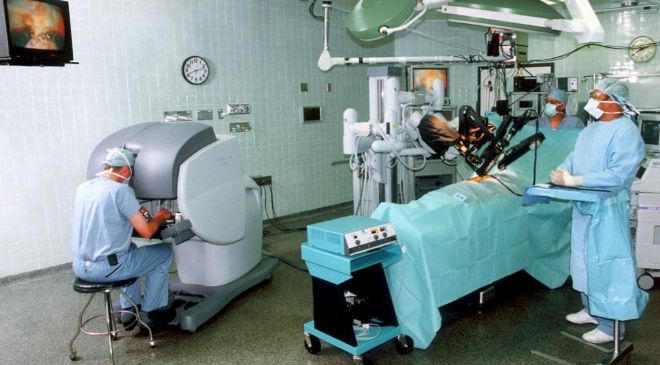
\includegraphics[width=0.8\textwidth]{figures/sistemadavinci.jpg}
		\caption{Sistema Da Vinci}
		\label{fig.sistemadavinci}
		\end{center}
\end{figure}
\item Industria: Probablemente se trate del sector donde más extendido este el uso de la robótica, desde mover una pieza de posición hasta cargar y descargar el maquinas. Sin embargo, hay una industria donde sobresale por encima del resto: el sector del automóvil. En España, según datos de la Asociación Española de Robótica, seis de cada diez robots pertenecen a este sector. Los robots se encargan de distribuir por toda una fabrica los componentes necesarios, así como posteriormente montarlos. Gracias a la robotización de la industrias, la producción ha aumentado en los últimos años de manera significativa, disminuyendo costes y errores.
\begin{figure}[H]
  \begin{center}
    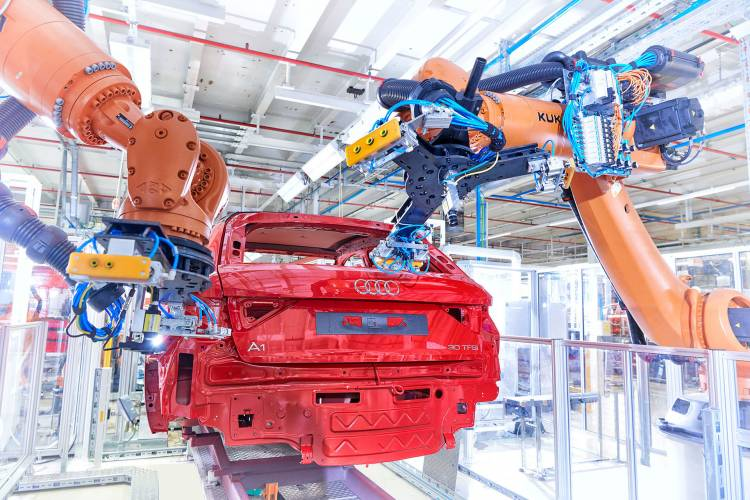
\includegraphics[width=0.8\textwidth]{figures/robotautomovil.jpg}
		\caption{Fábrica de Seat en Martorell}
		\label{fig.robotautomovil}
		\end{center}
\end{figure}
\item Militar: Si la industria es el sector donde más se utiliza la robótica, sin lugar a duda el sector militar es donde más dinero se invierte y se investiga. Actualmente hay multitud de robots usados militarmente como los vehículos aéreos no tripulados Hermes y Predator, el Goalkeeper CIWS, que es un sistema de armamento defensivo por proximidad holandés, o Samsung SGR-A1, que es un robot centinela utilizado para la vigilancia de la zona desmilitarizada entre Corea del Sur y Corea del Norte. Sin embargo, actualmente la investigación esta centrada en la elaboración de un robot humanoide capaz de caminar por terrenos irregulares y zonas catastróficas para realizar tareas de rescate y ayuda humanitaria. En este sentido, entre el año 2012 y 2015, el Departamento de Defensa de Estados Unidos, a través de su Agencia de Proyectos  de Investigación Avanzada en Defensa (DARPA)., creó una competición con el objetivo de desarrollar robots terrestres semiautónomos capaces de realizar tareas complejas en entornos peligrosos y degradados \footnote{\url{https://www.darpa.mil/program/darpa-robotics-challenge}}. El premio fue ganado por el robot humanoide desarrollado por el Instituto Avanzado de Ciencia y Tecnología de Corea, ``DRC-Hubo''.
\begin{figure}[H]
  \begin{center}
    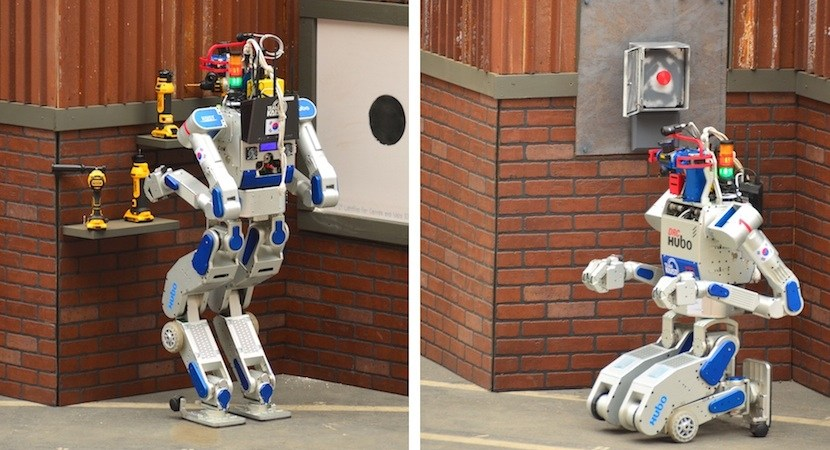
\includegraphics[width=0.8\textwidth]{figures/drchubo.jpg}
		\caption{Robot DRC-Hubo durante el DARPA Robotics Challenge}
		\label{fig.drchubo}
		\end{center}
\end{figure}
\end{itemize}

\subsection{Software para el desarrollo de componentes robóticos}

El software es el encargado de proporcionar al robot la inteligencia y autonomía necesaria para que realice las funciones o acciones que deseamos. Para facilitar esta tarea, se han creado middleware y bibliotecas especificas.

\subsubsection{Middleware}

Un robot es un sistema complejo ya que es un conjunto de diferentes componentes hardware y software (sensores, actuadores, etc.). Para cada robot, sería necesario un software personalizado que sea capaz de: leer y extraer la información necesaria de cada uno de los sensores, calcular y enviar las secuencias de acciones para que realice una determinada tarea o acción, controlar los actuadores, etc. Desarrollar este software se vuelve una tarea compleja e inútil dado que por lo general, si cambiáramos de robot este software no funcionaría de manera correcta.
En este escenario es donde un middleware nos proporcionará las herramientas que necesitamos para facilitar en gran medida la labor, ya que nos permitirá estructurar el software separando las diferentes tares (lectura de sensores, extracción de datos, especificar la velocidad, etc.) y haciendo exportable el uso de este software con cualquier otro sistema robótico al tener un marco común de comunicación gracias al middleware.
Actualmente hay una gran cantidad de middleware que permiten esta abstracción, siendo algunos de los más destacados los que señalo a continuación:
\begin{itemize}
	\item Robot Operating System (ROS)\footnote{\url{http://www.ros.org/}}: Pese a ser un middleware, se podría decir que ROS pretende ser algo más. Nos provee de la funcionalidad que cabría esperar de un sistema operativo (abstracción del hardware, control de dispositivos de bajo nivel, la trasferencia de mensajes entre procesos, administración de paquetes, etc.). El principal objetivo es permitir la reutilización del código en la investigación y desarrollo de robótica, lanzando paquetes de software que están listos para ser usados por cualquier desarrollador. ROS cuenta con una gran comunidad de colaboradores, que comparten sus paquetes y proyectos, gracias a su sitio web y repositorios.
	\item Internet Communication Engine (ICE) \footnote{\url{https://zeroc.com/}}: Creado por la empresa ZeroC, se trata de un middleware orientado a objetos que permite la creación de aplicaciones multilenguaje y multiplataforma, permitiendo la comunicación con diferentes arquitecturas de red (UDP, TCP, WebSockets, etc.). ICE no es un middleware robótico propiamente dicho, pero su uso facilita el desarrollo de la conectividad con sistemas robóticos, al permitirnos crear nuestras propias interfaces para el intercambio de datos.
	\item Open Robot Control Software project (Orocos) \footnote{\url{http://www.orocos.org/}}: Se trata de un proyecto de software libre cuyo objetivo es la creación de un paquete de software para el control de robots.
	\item Orca \footnote{\url{https://www.orcaconfig.com/}}: Se trata de un middleware de código libre que se originó a partir del proyecto Orocos. Orca está diseñado para desarrollar sistemas robóticos basados en componentes. Su principal objetivo es permitir, facilitar y simplificar la reutilización del código entre desarrolladores.
	\item Middleware for Robots (Miro): Se trata de un middleware orientado a objetos para el control de robots móviles, y basado en CORBA (Common Object Request Broker Architecture). El hecho de que sea orientado a objetos permite la interoperabilidad entre procesos y plataformas cruzadas para el control de robots distribuidos.
	\item JdeRobot \footnote{\url{https://jderobot.org/}}: Se trata de una plataforma de código abierto para el desarrollo de aplicaciones de visión artificial y robóticas, compatible con middlewares de comunicación ICE y ROS y desarrolladas principalmente en Python y C++.
\end{itemize}

\subsubsection{Bibliotecas}

En programación, una biblioteca es una colección de recursos utilizados para el desarrollo de software. Hay multitud de bibliotecas para el desarrollo de sistemas robóticos: bibliotecas para procesar imágenes, interactuar con el robot, procesar elementos 3D, etc. Las bibliotecas más utilizadas son:
\begin{itemize}
	\item OpenCV \footnote{\url{https://opencv.org/}}: Es la biblioteca de visión artificial por excelencia. Creada originalmente por Intel, es de código abierto y desarrollada en C++. Actualmente dispone de interfaces en C++, C, Python, Java y están empezando a desarrollar para JavaScript.
	\item Point Cloud Library (PCL) \footnote{\url{http://pointclouds.org/}}: Se trata de una biblioteca de código abierto que proporciona algoritmos para el procesamiento de nubes de puntos y geometría 3D.
	\item Bibliotecas de ROS: ROS proporciona bibliotecas para cada lenguaje de programación al que da soporte, ofreciendo una serie de funciones y algoritmos que nos permite crear aplicaciones que interactúan rápidamente con ROS. Las bibliotecas más utilizadas son rospy \footnote{\url{http://wiki.ros.org/rospy}}, que está desarrollada para Python y roscpp \footnote{\url{http://wiki.ros.org/roscpp}}, que está desarrollada para ser usada con C++. Cabe destacada, también, la biblioteca roslibjs, que ofrece las funcionalidades para JavaScript.
\end{itemize}

\subsubsection{Simuladores}

Un simulador robótico nos permite imitar el funcionamiento de un sistema robótico para poder probar las aplicaciones, evitando que surjan fallos críticos a la hora de hacerlo funcionar con el sistema real. Estos fallos pueden conllevar averías muy costosas a nivel monetario y de tiempo, que conllevarían retrasos importantes a la hora de realizar el desarrollo. Los simuladores más utilizados son:
\begin{itemize}
	\item Gazebo \footnote{\url{http://gazebosim.org/}}: Se trata de uno de los simuladores más utilizados en la actualizada gracias a su fácil manejo y su intuitiva interface. Gazebo es un simulador de código abierto que ofrece múltiples motores de físicas, motores de renderizado avanzado, soporte para plug-ins y programación en la nube. Además, dispone de un gran número de robots, sensores y cámaras para simular, lo que permite realizar las pruebas de nuestras aplicaciones de forma bastante realista y, así poder utilizar nuestra aplicación con el sistema físico sin miedo a que sufra daños.
	\item ROS Development Studio (RDS \footnote{\url{http://www.theconstructsim.com/}}): Elaborado por la empresa española TheConstruct, se trata de un simulador web que permite simulador sistemas robóticos, a la vez que ofrece un editor y una consola para poder crear nuestro código, pero únicamente ofrece soporte para Python gracias a Jupyter. La gran ventaja que ofrece este simulador es que no es necesario realizar ninguna instalación, simplemente registrarte en su página web y acceder con un navegador. Ofrecen desde una versión básica gratuita hasta una versión para expertos con una tarifa mensual.
\end{itemize}
Existen otros simuladores como son Stage para la simulación en 2D o  Webots, pero no tan utilizados como Gazebo o sin las ventajas de RDS.

\section{Tecnologías web}
Desde que en el año 1992, Tim Berners-Lee ideara y desarrollara las primeras herramientas para facilitar compartir información entre los científicos del CERN desde cualquier parte del mundo, dando lugar a la posteriormente llamada World Wide Web o como se conoce coloquialmente la web, ha sufrido una gran evolución, consiguiendo que la sociedad actual no se pueda entender sin la existencia de la misma. Sin embargo, pese a la gran evolución, el propósito de la web no ha cambiado, es decir, que acceder a la información sea lo más fácil posible. Sí lo ha hecho la manera en que la utilizamos. La aparición de aplicaciones web como las redes sociales, los servicios de streaming o los comercios electrónicos, han supuesto un impulso importante en el uso de la web y, por consiguiente, la necesidad de idear nuevas herramientas que faciliten el desarrollo de webs.

\subsection{Arquitectura de una aplicación web}
Desde su creación, el modelo para que un sitio o aplicación web funcione no ha variado.
\begin{itemize}
	\item Cliente: Realiza las peticiones de recursos a diferentes servidores web a través de un localizador uniforme de recursos (URL). Generalmente, la función de cliente la realizada un navegador.
	\item Servidor: Almacena la información de la aplicación web y sirve los contenidos acorde a las peticiones realizadas por el navegador.
	\item Http: Es el protocolo creado por Bernens-Lee que permite el intercambio de información entre el cliente y el servidor.
\end{itemize}
\begin{figure}[H]
  \begin{center}
    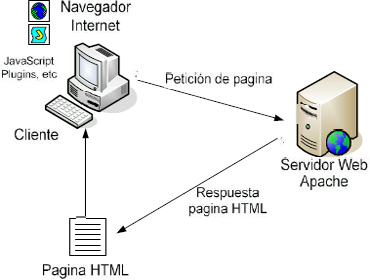
\includegraphics[width=0.8\textwidth]{figures/arquitecturaweb.jpg}
		\caption{Arquitectura de una aplicación web}
		\label{fig.arquitecturaweb}
		\end{center}
\end{figure}

\subsection{Tecnologías del lado del cliente}
Estas tecnologías son las encargadas de dar forma a la interfaz de usuario y de establecer la comunicación con el servidor. El navegador es capaz de leer e interpretar estas tecnologías. Las más utilizadas son las siguientes:
\begin{itemize}
	\item Hyper-Text Markup Lenguage (HTML): Es el lenguaje de descripción de aplicaciones web que nos permite especificar las características visuales.
	\item Hojas de estilo en cascada (CSS): Es el lenguaje utilizado para describir la presentación semántica (el aspecto y el formato) de un documento en lenguaje de marcas.
	\item JavaScript: Es un lenguaje de script orientado a objetos y guiado por eventos que nos permiten realizar acciones en el cliente e interactuar con el servidor u otras aplicaciones web.
\end{itemize}

\subsection{Tecnologías del lado del servidor}
Estas tecnologías son las encargadas de dar forma al servidor web de manera que permita el acceso a bases de datos, conexiones de red, recursos compartidos, en definitiva, se encarga de realizar todas las tareas necesarias para crear la aplicación web que se visualizará en el cliente. Las tecnologías más utilizadas son las siguientes:
\begin{itemize}
	\item Common Gatewey Interface (CGI): Fue de las primeras tecnologías del lado del servidor en aparecer, se creó inicialmente para gestionar formularios. No se trata de un lenguaje de programación sino  de un mecanismo de comunicación entre el cliente y un programa externo, que proporcionará el contenido de la aplicación web. Actualmente se utiliza una variante llamada Fast-CGI que proporciona una mayor rapidez.
	\item PHP: Creado en 1994, es la tecnología más utilizada. Se trata de un lenguaje de programación de uso general de script que originalmente fue diseñado para proporcionar contenido web dinámico. Su código está empotrado en el código HTML y es interpretado por un servidor web para generar la aplicación web, evitando la necesidad de acceder a un archivo externo.
	\item Servlets: Son programas escritos en Java que se ejecutan sobre un servidor de aplicaciones mediante la maquina virtual de Java (JVM). Estos programas (servlets) son ejecutados por el servidor para manejar cada una de las peticiones del cliente. Se trata de una tecnología con un concepto similar a CGI, pero beneficiándose de las ventajas de el entorno Java.
	\item JavaServer Pages (JSP):Se trata de una tecnología Java que permite generar contenido web dinámico en forma de documentos HTML. El código Java, a diferencia que en los Servlets, va incrustado en el HTML y se compila dinámicamente como un servlet.
	\item Active Server Page (ASP): Creado por Microsoft en 1996. Se trata de código que se ejecuta en el servidor y genera un archivo HTML que devuelve al cliente. Al ser una tecnología creada por Microsoft, permite la compatibilidad con componentes ActiveX (acceso a base de datos, scripts, etc.) lo que proporciona una gran potencia y flexibilidad. Esta tecnología solo puede ser utilizada en servidores con sistemas operativos de Microsoft.
	\item Python, Django: Se trata de un framework programado en Python que proporciona un conjunto de componentes en el lado del servidor para ayudar a la hora de desarrollar una aplicación web. Sigue el diseño de Modelo-Vista-Controlador, que se trata de un modelo que separa la lógica y datos de la interfaz gráfica y de las comunicaciones y eventos. Cuando un cliente solicita una URL al servidor, esta pasa por Django que analizará la URL solicitada y pasará la petición a la función correspondiente llamada vista. En esta función se ejecutará lo necesario para proporcionar al cliente lo solicitado con su URL.
	\item Ruby on Rails: Al igual que Django, Ruby on Rails se trata de un framework para facilitar el desarrollador web programado en Ruby que sigue el diseño de Modelo-Vista-Controlador. El funcionamiento de Django y Rails es muy similar, siendo la principal diferencia el lenguaje en el que están programados, siendo necesario menos código en el caso de Rails.
	\item Node.js: Se trata de un entorno de ejecución multiplataforma de código abierto para el lado del servidor basándose en el lenguaje JavaScript. Este entorno se basa en eventos y gestiona todas las operaciones con una programación asíncrona. Todo esto facilita el desarrollo de aplicaciones web escalables de manera sencilla y con robustas.
\end{itemize}

\subsection{Tecnologías web en la actualidad}
Actualmente, el uso de tecnologías web está muy extendido, no concibiendo la vida moderna sin ellas. Las redes sociales, tiendas online, servicios de streaming, etc, son utilizados en multitud de ocasiones a lo largo de nuestro día a día. A continuación se mostrará algunos ejemplos de aplicaciones y paginas web más utilizadas:
\begin{itemize}
\item Spotify\footnote{\url{https://www.spotify.com/es/}}: Aplicación creada para la reproducción de música vía streaming, actualmente cuenta con más de 75 millones de usuarios activos convirtiéndose en una de las principales formas de escuchar música en la actualidad. La aplicación esta desarrollada mediante JavaScript (lado del cliente) y Python (lado del servidor).
\item Facebook\footnote{\url{https://es-es.facebook.com/}}: Se trata de la red social más conocida y que provoco el auge de las mismas, actualmente cuenta con más de 2200 millones de usuarios. Originalmente nació como una página web desarrollada mediante HTML y JavaScript para el lado del cliente y PHP para el lado del servidor, ha evolucionado hasta disponer una aplicación que puede ser utilizada en nuestros teléfonos móviles.
\item Google maps\footnote{\url{https://www.google.es/maps}}: Se trata de un servicio de mapas que permite desplazarse por el mundo, ver fotografías por satélite o recorrer una ubicación a pie de calle. Actualmente es utilizada para indicar ubicaciones, a modo de GPS o para encontrar lugares de interés, convirtiéndose en un sistema de referencia en la sociedad de hoy en día ya que se envían ubicaciones a través de esta aplicación de manera constante. La base de esta aplicación es JavaScript, usando HTML y CSS para la interfaz gráfica.
\item YouTube\footnote{\url{https://www.youtube.com/}}: Aplicación y página web dedicado a la compartición de videos entre usuarios. Actualmente, cuenta con más de 1900 millones de usuarios al mes y cada minuto se suben más de 120 horas de vídeo, llegando a convertirse en un oficio para miles de personas que ganan dinero publicando sus propios videos comentando videojuegos, consejos o criticas de multitud de cosas (móviles, películas, juguetes, etc.). YouTube está desarrollado mediante JavaScript y HTML en el lado del cliente y Python en el lado del servidor, incluso proporciono el primer reproductor de video incrustado en el HTML, que posteriormente fue incluido por el World Wide Web Consortium.
\item Whatsapp\footnote{\url{https://www.whatsapp.com/}}: Es una aplicación de mensajería instantánea que permite el intercambio entre usuario de mensajes a través de internet sin coste adicional. Cuenta con más de mil millones de usuario actualmente, ha supuesto una revolución al provocar la extinción del servicio de mensajes cortos (SMS) que conllevaban un coste mensual alto en beneficio de las operadoras móviles. Tras ser usado como aplicación, en el año 2015 se lanzó la versión web de Whatsapp para su usó en un ordenador, provocando que la aplicación de mensajería de Google, Hangouts, sufriera una reducción importante de usuarios, siendo uno de los factores que ha llevado a Google a anunciar el cierre del servicio en el año 2020.
\end{itemize}

\section{Tecnologías web en robótica}

La utilización de tecnologías web en robótica es aún, pese a su aumento en los últimos tiempos, un campo con poco desarrollo. Sin embargo, debido a las ventajas que ofrece frente a otras tecnologías (el mismo código funciona en cualquier plataforma, no es necesario realizar ninguna instalación, etc.) es un campo prometedor de cara al futuro.

Como se ha mencionado anteriormente, aún no hay muchos desarrollos basados en tecnologías web, siendo el más importante de ellos las bibliotecas y herramientas de código abierto para su utilización con el middleware ROS, elaboradas por la comunidad de Robot Web Tools \footnote{\url{http://robotwebtools.org/}}.
Los desarrollos más importantes que han realizado son:
\begin{itemize}
	\item Rosbridge Suite: Proporciona una interfaz usando JSON para ROS que permite a cualquier cliente enviar JSON para conectarnos con el robot, mediante las capas de comunicación WebSockets, UDP y TCP. Realmente podría entenderse como un servidor intermedio que recibe o envía la información a un cliente web.
	\item roslibjs: Se trata de la biblioteca que da soporte a la interactuación entre una aplicación web desarrollada en JavaScript con ROS. 
	\item ros2djs y ros3djs: Son las bibliotecas elaboradas para gestionar la visualización de elementos en dos y tres dimensiones, respectivamente. Están elaboradas utilizando roslibjs y proporcionan funciones que son estándares en ROS como la elaboración de mapas, el procesado de nubes de puntos o del escaneo laser.
\end{itemize}

Adicionalmente, ofrecen una serie de herramientas como son un servidor de video web, una herramienta para mostrar e interactuar con la navegación autónoma del robot, una herramienta para la creación de teleoperadores de robots, etc.

\section{Trabajos Previos}
Una parte de este proyecto está basado en el TFG elaborado por Aitor Martínez \footnote{\url{https://jderobot.org/Aitormf-tfg}}. En este trabajó, utilizando tecnologías web, se crearon tres aplicaciones que eran capaces de conectarse con varios sistemas robóticos. El resto del proyecto se basará en la adaptación a tecnologías web del visor 3D y del servidor de imágenes desarrollados con C++ de la plataforma JdeRobot.

\subsection{CameraViewjs}

Se trata de un visualizador de imágenes, desarrollado utilizando JavaScript, HTML5 y CSS3 en el lado del Cliente y NodeJS en el lado del servidor, e ICE como middleware. Esta aplicación permite la visualización de las imágenes recibidas desde un servidor de imágenes, ya sean obtenidas desde una webcam, una cámara conectada a un robot o almacenadas en el dispositivo.

\begin{figure}[H]
  \begin{center}
    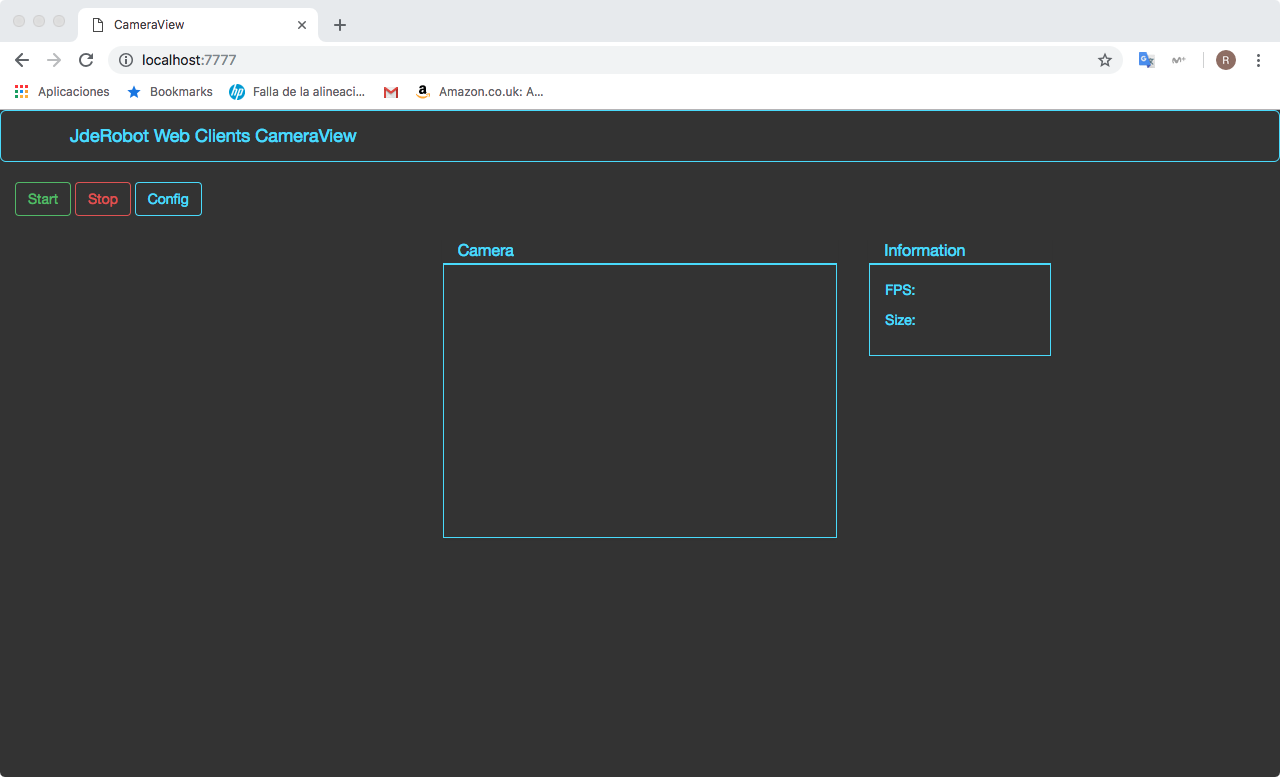
\includegraphics[width=0.8\textwidth]{figures/cameraviewjs.png}
		\caption{CameraViewjs}
		\label{fig.cameraviewjs}
		\end{center}
\end{figure}

\subsection{KobukiViewerjs}

Se trata de un visualizador y teleoperador de robots del tipo Turtlebot, desarrollado utilizando JavaScript, HTML5 y CSS3 en el lado del Cliente y NodeJS en el lado del servidor, e ICE como middleware. Consta de varias partes, la primera de ellas es mostrar las imágenes obtenida a través de las dos cámaras de las que dispone el robot (izquierda y derecha), otra parte donde muestra la imagen del escaneo láser obtenida, una representación tridimensional del robot y el movimiento del mismo, y por último, el teleoperador, que envía al robot una velocidad lineal y otra angular para indicar tanto el movimiento en linear recta como la orientación del mismo.

\begin{figure}[H]
  \begin{center}
    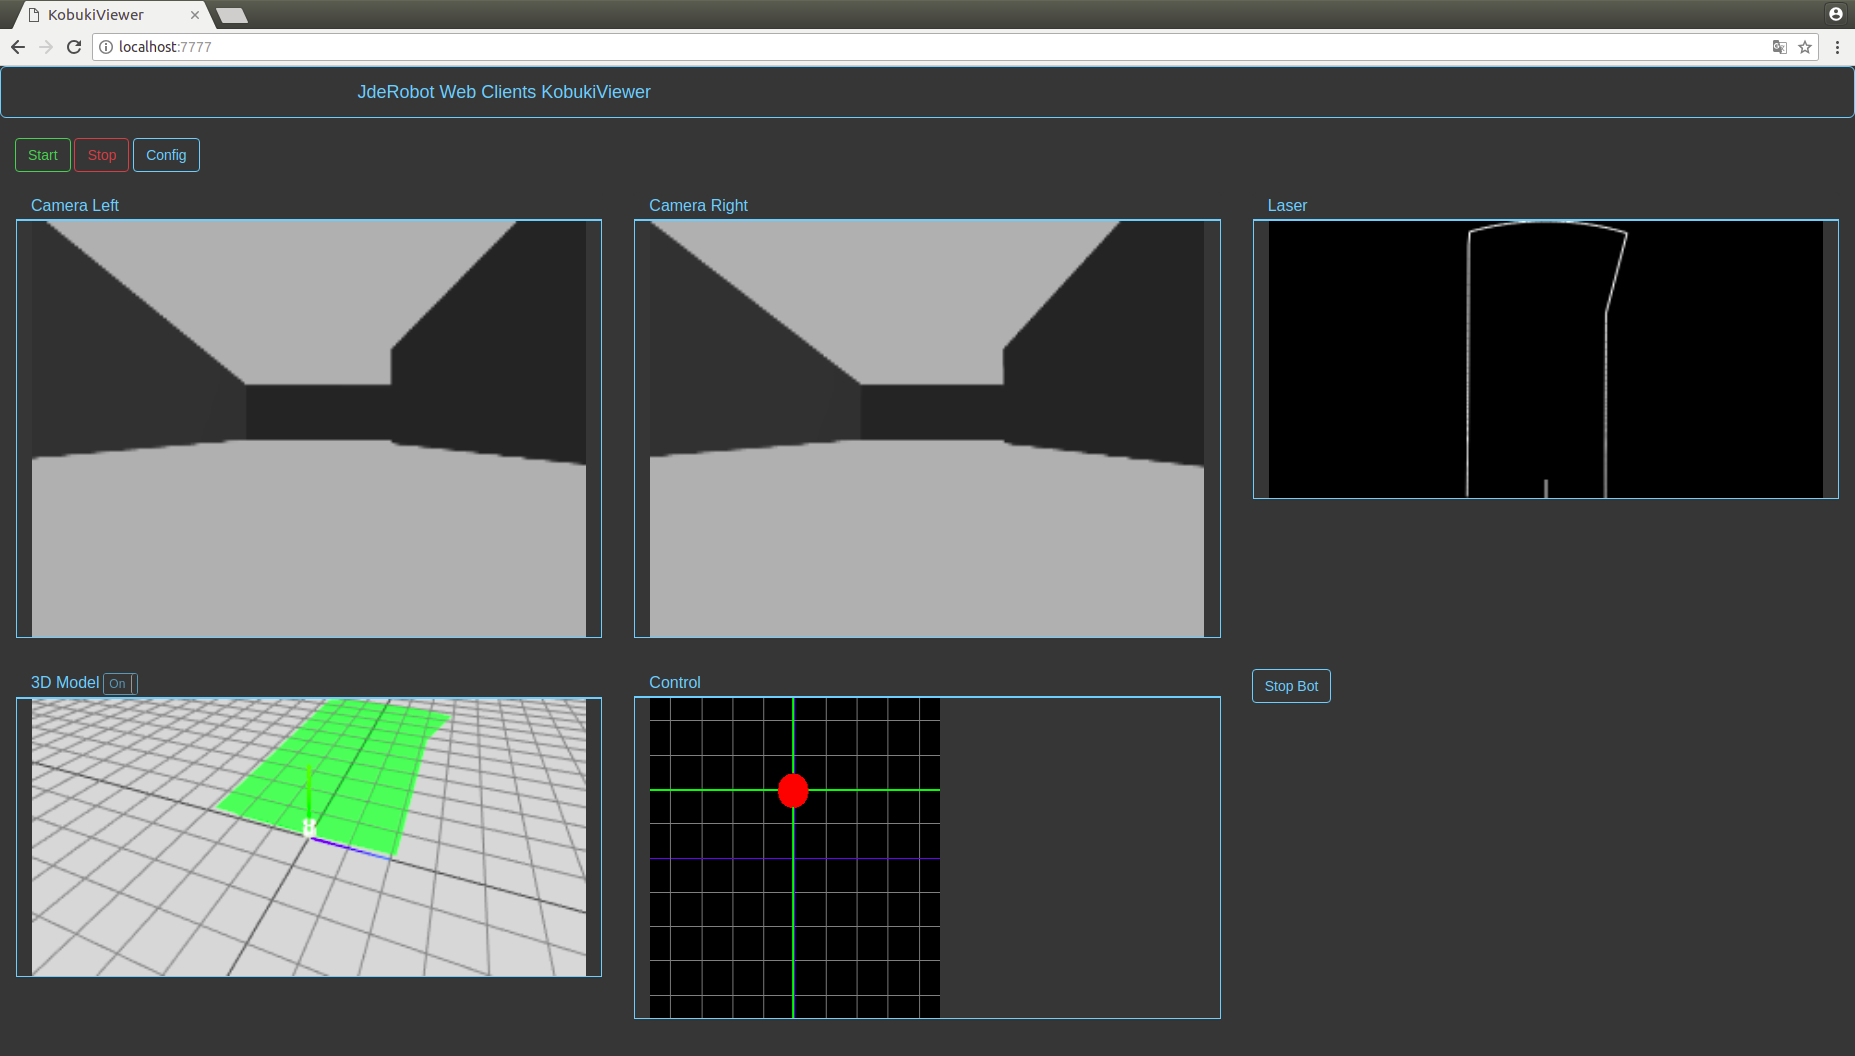
\includegraphics[width=0.8\textwidth]{figures/kobukiviewerjs.png}
		\caption{KobukiViewerjs}
		\label{fig.kobukiviewerjs}
		\end{center}
\end{figure}

\subsection{UavViewerjs}

Se trata de un visualizador y teleoperador de drones, desarrollado utilizando JavaScript, HTML5 y CSS3 en el lado del Cliente y NodeJS en el lado del servidor, e ICE como middleware. La aplicación tiene integrada sobre la misma pantalla el teleoperador y la imagen obtenida de la cámara, pudiéndose elegir si deseamos mostrar la cámara frontal o de abajo del dron. Consta también de una representación tridimensional del dron y de su movimiento. Desde la aplicación se teleopera mediante él envió de una velocidad lineal y otra angular, además se le indica cuando se desea aterrizar y despegar.

\begin{figure}[H]
  \begin{center}
    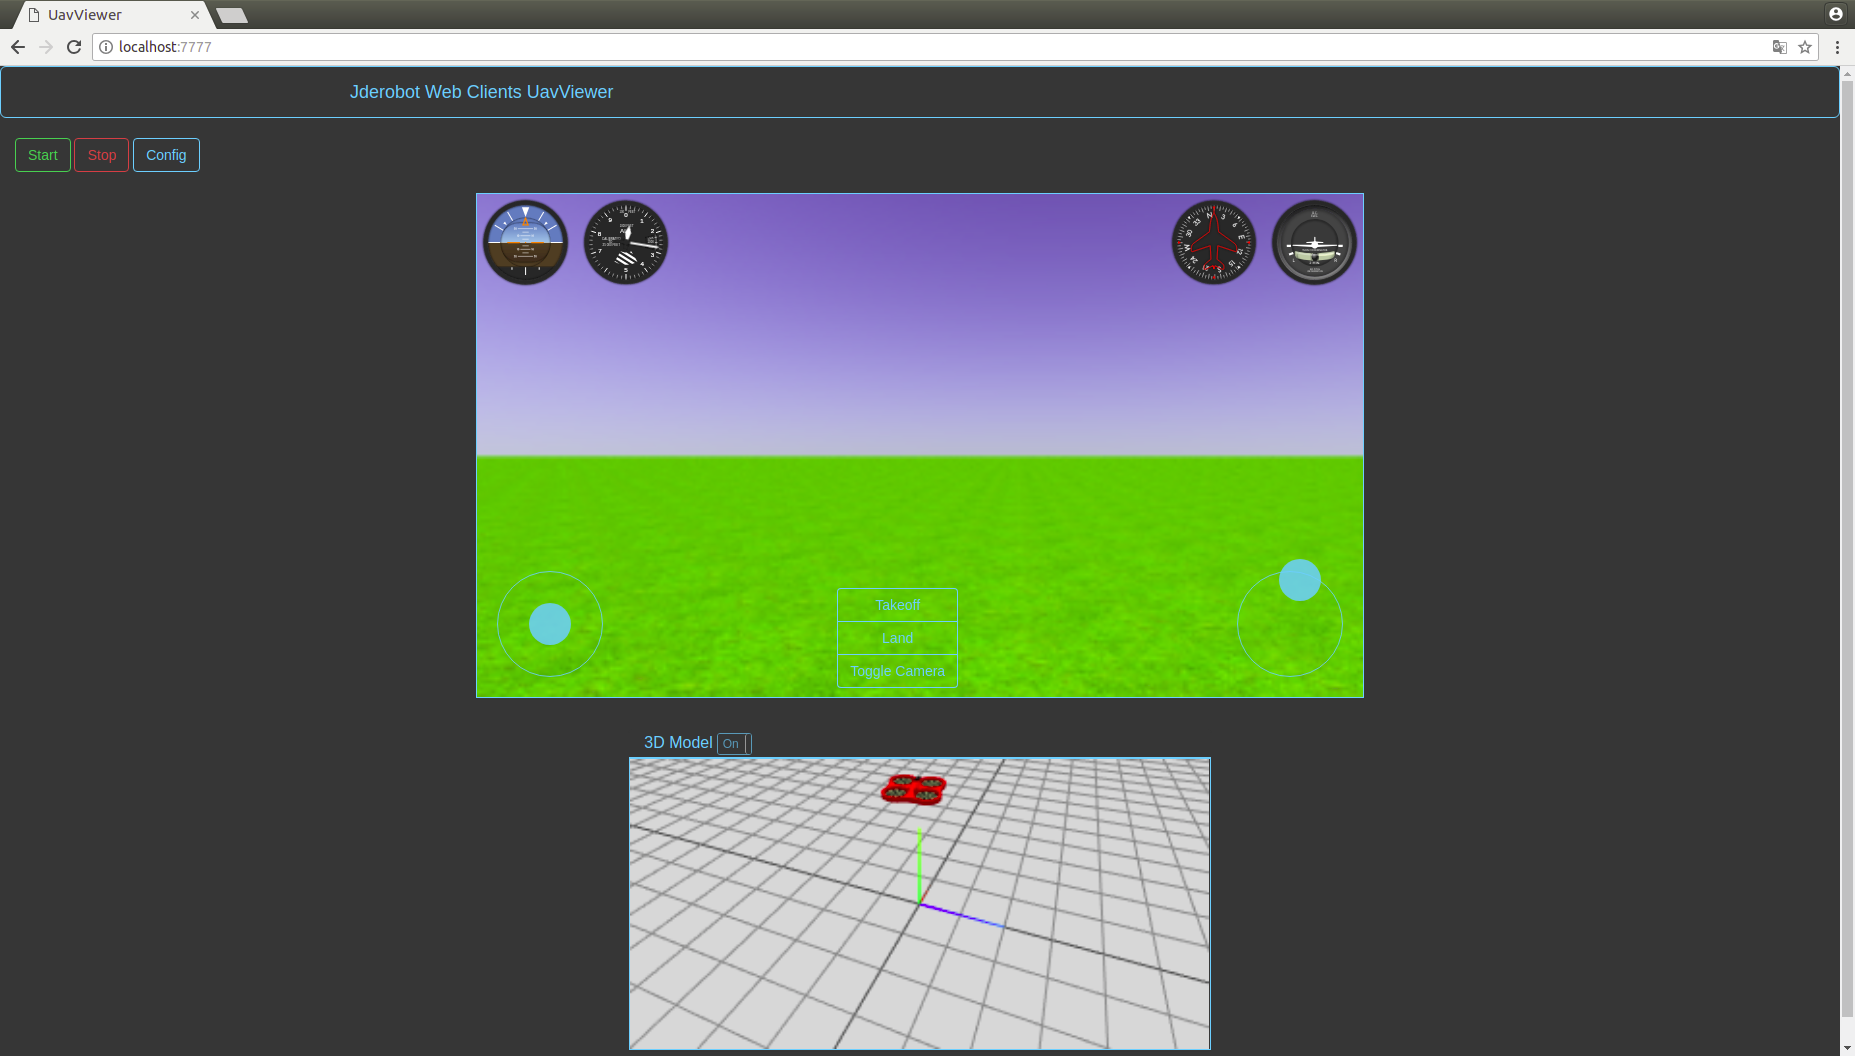
\includegraphics[width=0.8\textwidth]{figures/uavviewerjs.png}
		\caption{UavViewerjs}
		\label{fig.uavviewerjs}
		\end{center}
\end{figure}

\subsection{3DViewer}
3DViewer \footnote{\url{https://jderobot.org/Tools}} es la herramienta para visualizar puntos 3D de la plataforma JdeRobot. Este visor es utilizado conjuntamente con la práctica de JdeRobot Academy de reconstrucción 3D \footnote{\url{https://jderobot.org/JdeRobot-Academy}} para reconstruir mediante puntos de la imagen obtenida con un par de cámaras RGB.

\begin{figure}[H]
  \begin{center}
    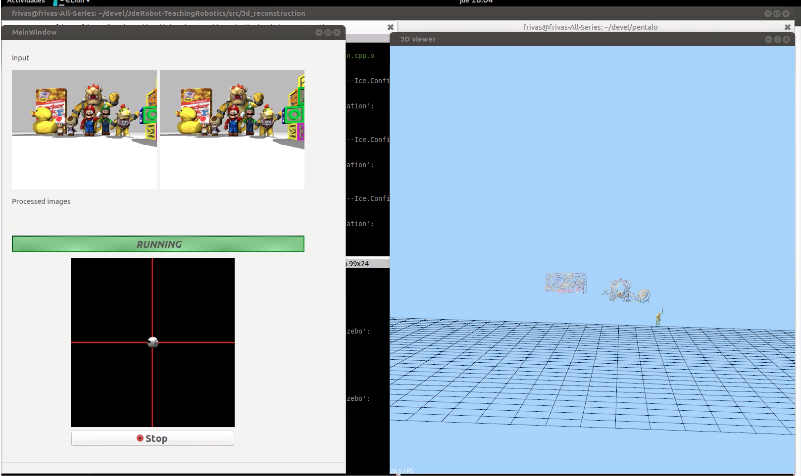
\includegraphics[width=0.8\textwidth]{figures/3DViewer.png}
		\caption{3DViewer usado con la práctica de JdeRobot Academy}
		\label{fig.3DViewer}
		\end{center}
\end{figure}
\subsection{Cameraserver}
Cameraserver \footnote{\url{https://jderobot.org/Handbook}} es el componente de la plataforma JdeRobot que sirve las imágenes obtenidas a través de una fuente de video, real o simulada, y transmitidas mediante del middleware ICE para su visualización por parte de uno o varios clientes.
